\documentclass{math}

\usepackage{graphicx}

\title{Principles of Data Mining: HW 00}
\author{Alvin Lin}
\date{August 2018 - December 2018}
\begin{document}

\maketitle

\subsection*{Task 1}
\begin{center}
  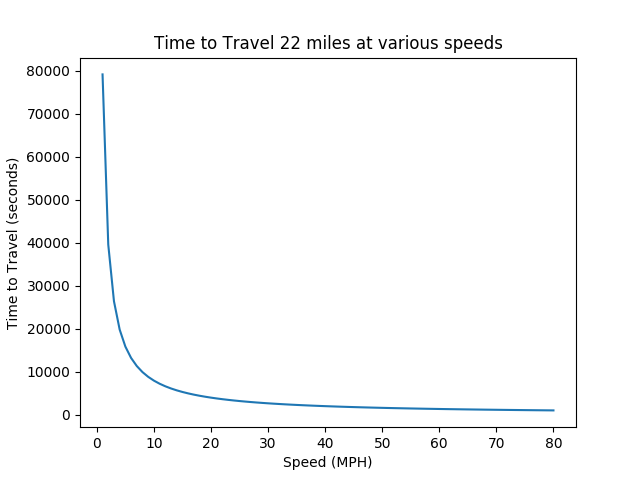
\includegraphics[width=15cm]{assets/hw_00_task1.png}
\end{center}

\subsection*{Task 2}
\begin{center}
  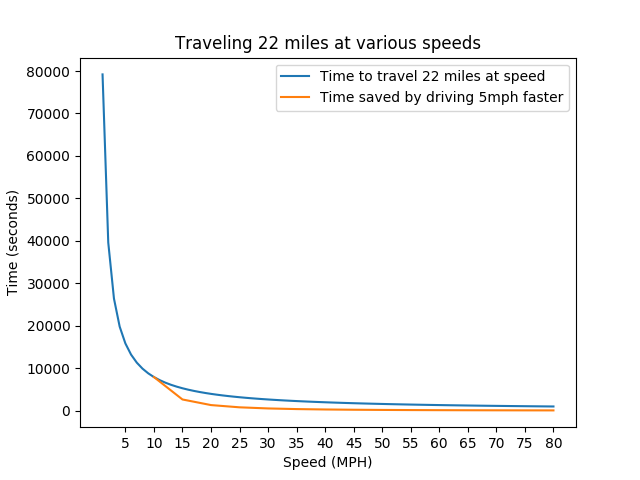
\includegraphics[width=15cm]{assets/hw_00_task2.png}
\end{center}

\subsection*{Task 3}
\begin{center}
  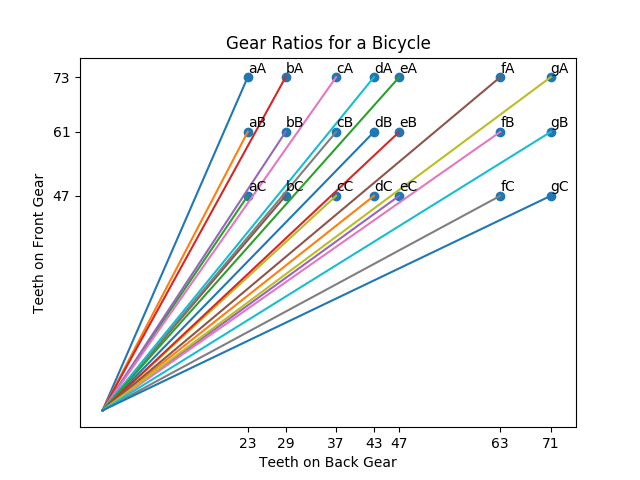
\includegraphics[width=15cm]{assets/hw_00_task3.png}
\end{center}

\subsection*{Task 4}
I chose this method for visualizing gear ratios because the slope of the line
drawn from (0,0) to the point representing the gear combination shows the gear
ratio. This allows us to easily compare the gear ratios of different gear
combinations simply by comparing the slope of the lines drawn. I did not try
using a number line, but I tried plotting this 3-dimensionally using the x axis
for the teeth on the back gear, the y axis for the teeth on the front gear, and
the z axis for the calculated gear ratio, but this was less obvious and
difficult to analyze.

\begin{center}
  If you have any questions, comments, or concerns, please contact me at
  alvin@omgimanerd.tech
\end{center}

\end{document}
